
%--- 幻灯片 1: 目录 ---
\begin{refsection}
    \begin{frame}{目录}
      \begin{itemize}
        \item 1. 基于深度学习的图像分类简介
        \item 2. 传统数据增强方法
        \item 3. 用于数据增强的生成模型
        \item 4. 灾害事件遥感数据集:xBD
      \end{itemize}
      \begin{itemize}
        \item 项目 - \textbf{探索生成图像是否能提升图像分类性能}
      \end{itemize}
    \end{frame}
\end{refsection}


\begin{refsection}
  \begin{frame}{图像分类:概述}
    \begin{figure}
      \centering
      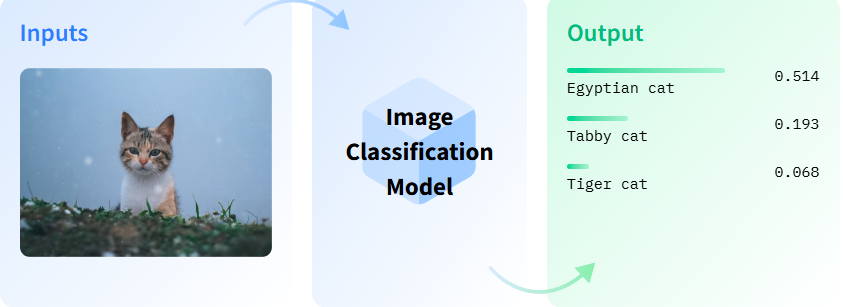
\includegraphics[height=0.65\textheight]{image_classification_idea.png}
      \caption{\scriptsize 图像分类的基本流程。}
    \end{figure}
    \bottomleftrefs
  \end{frame}
\end{refsection}

\begin{refsection}
  \begin{frame}{背景:深度学习下的图像分类}
    \begin{figure}
      \centering
      \begin{minipage}{0.48\linewidth}
        \centering
        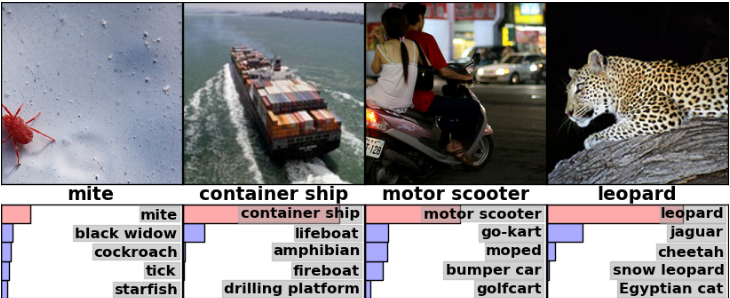
\includegraphics[width=\linewidth]{imagenet2.png}
      \end{minipage}\hfill
      \begin{minipage}{0.48\linewidth}
        \centering
        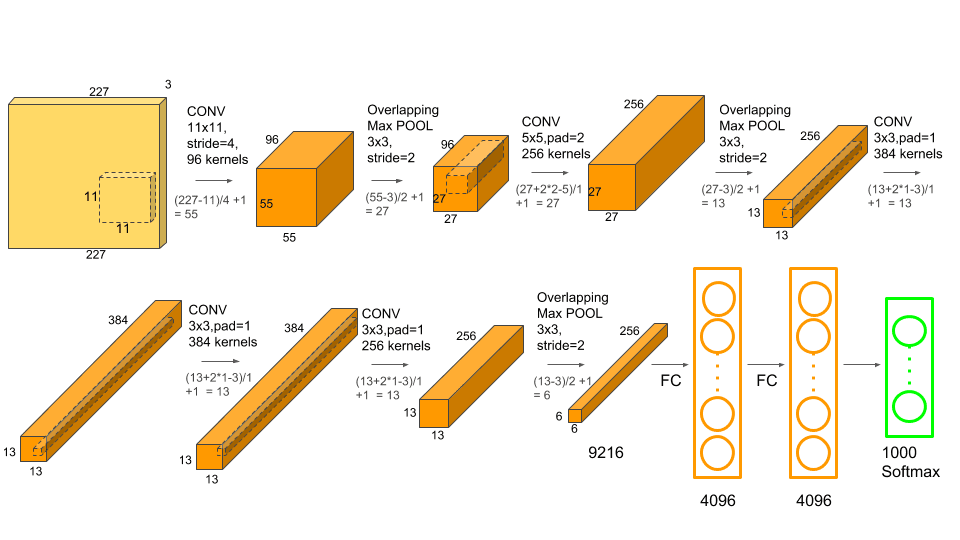
\includegraphics[width=\linewidth]{alexnet.png}
      \end{minipage}
      \caption[]{\scriptsize 左:AlexNet 在 ILSVRC-2010~\parencite{imagenet2010challenge} \quad 右:AlexNet 网络结构~\parencite{krizhevskyImageNetClassificationDeep2012}。}
    \end{figure}
    \bottomleftrefs
  \end{frame}
\end{refsection}

\begin{refsection}
  \begin{frame}{图像分类模型结构演进}
    \begin{minipage}{0.48\linewidth}
      {\small
      \begin{itemize}
        \item \textbf{2012: AlexNet}, \textbf{2016: ResNet}
        \item \textbf{2021: ViT}
        \item \textbf{2021: Swin Transformer} \\
        \parencite{liuSwinTransformerHierarchical2021}
        \parencite{dosovitskiyImageWorth16x162020}
        \item \textbf{2021: CLIP-ViT} \\
        \parencite{radfordLearningTransferableVisual2021}
        \item \textbf{2022: MAE-ViT} \\
        \parencite{heMaskedAutoencodersAre2022}
        \item \textbf{2022: CoCa-ViT} \\
        \parencite{yuCoCaContrastiveCaptioners2022}
      \end{itemize}
      }
    \end{minipage}%
    \hfill
    \begin{minipage}{0.48\linewidth}
      \centering
      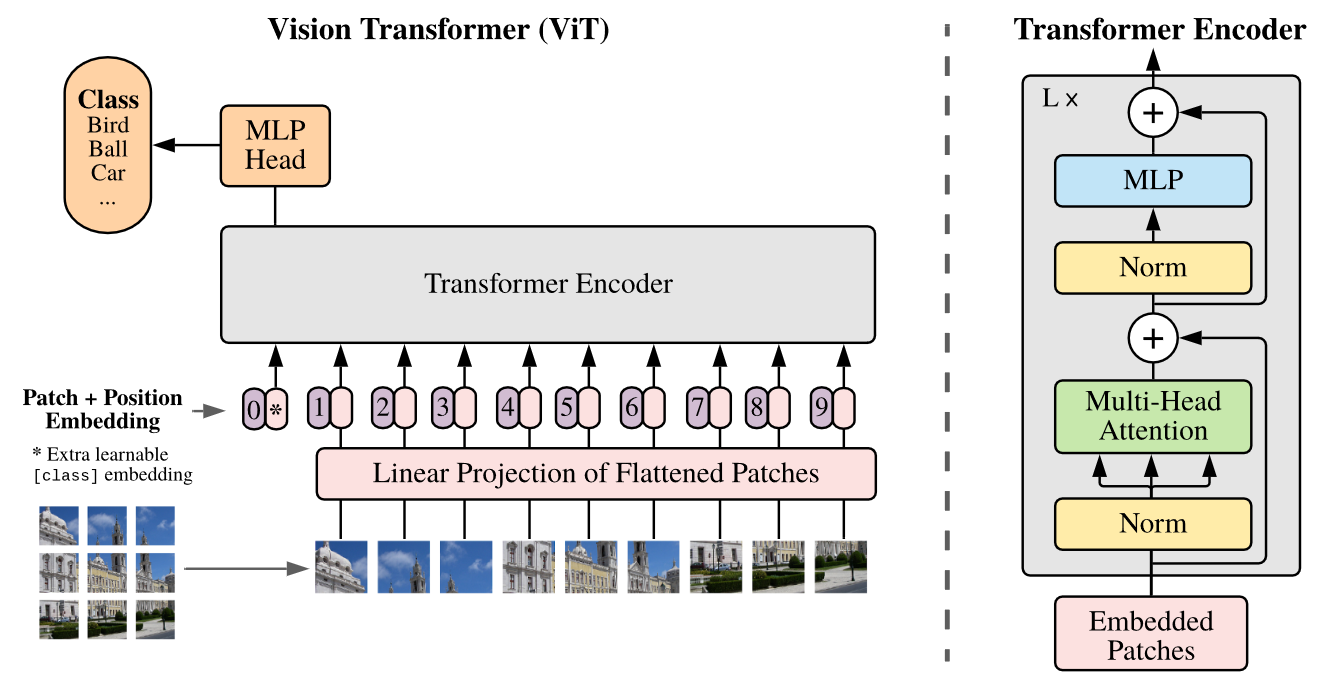
\includegraphics[width=0.95\linewidth]{vit.png}
      \scriptsize Vision Transformer 概览\\\parencite{dosovitskiyImageWorth16x162020}。
    \end{minipage}
    \bottomleftrefs
  \end{frame}
\end{refsection}

\begin{refsection}
  \begin{frame}{RemoteCLIP:遥感领域视觉-语言基础模型}
    \begin{figure}
      \centering
      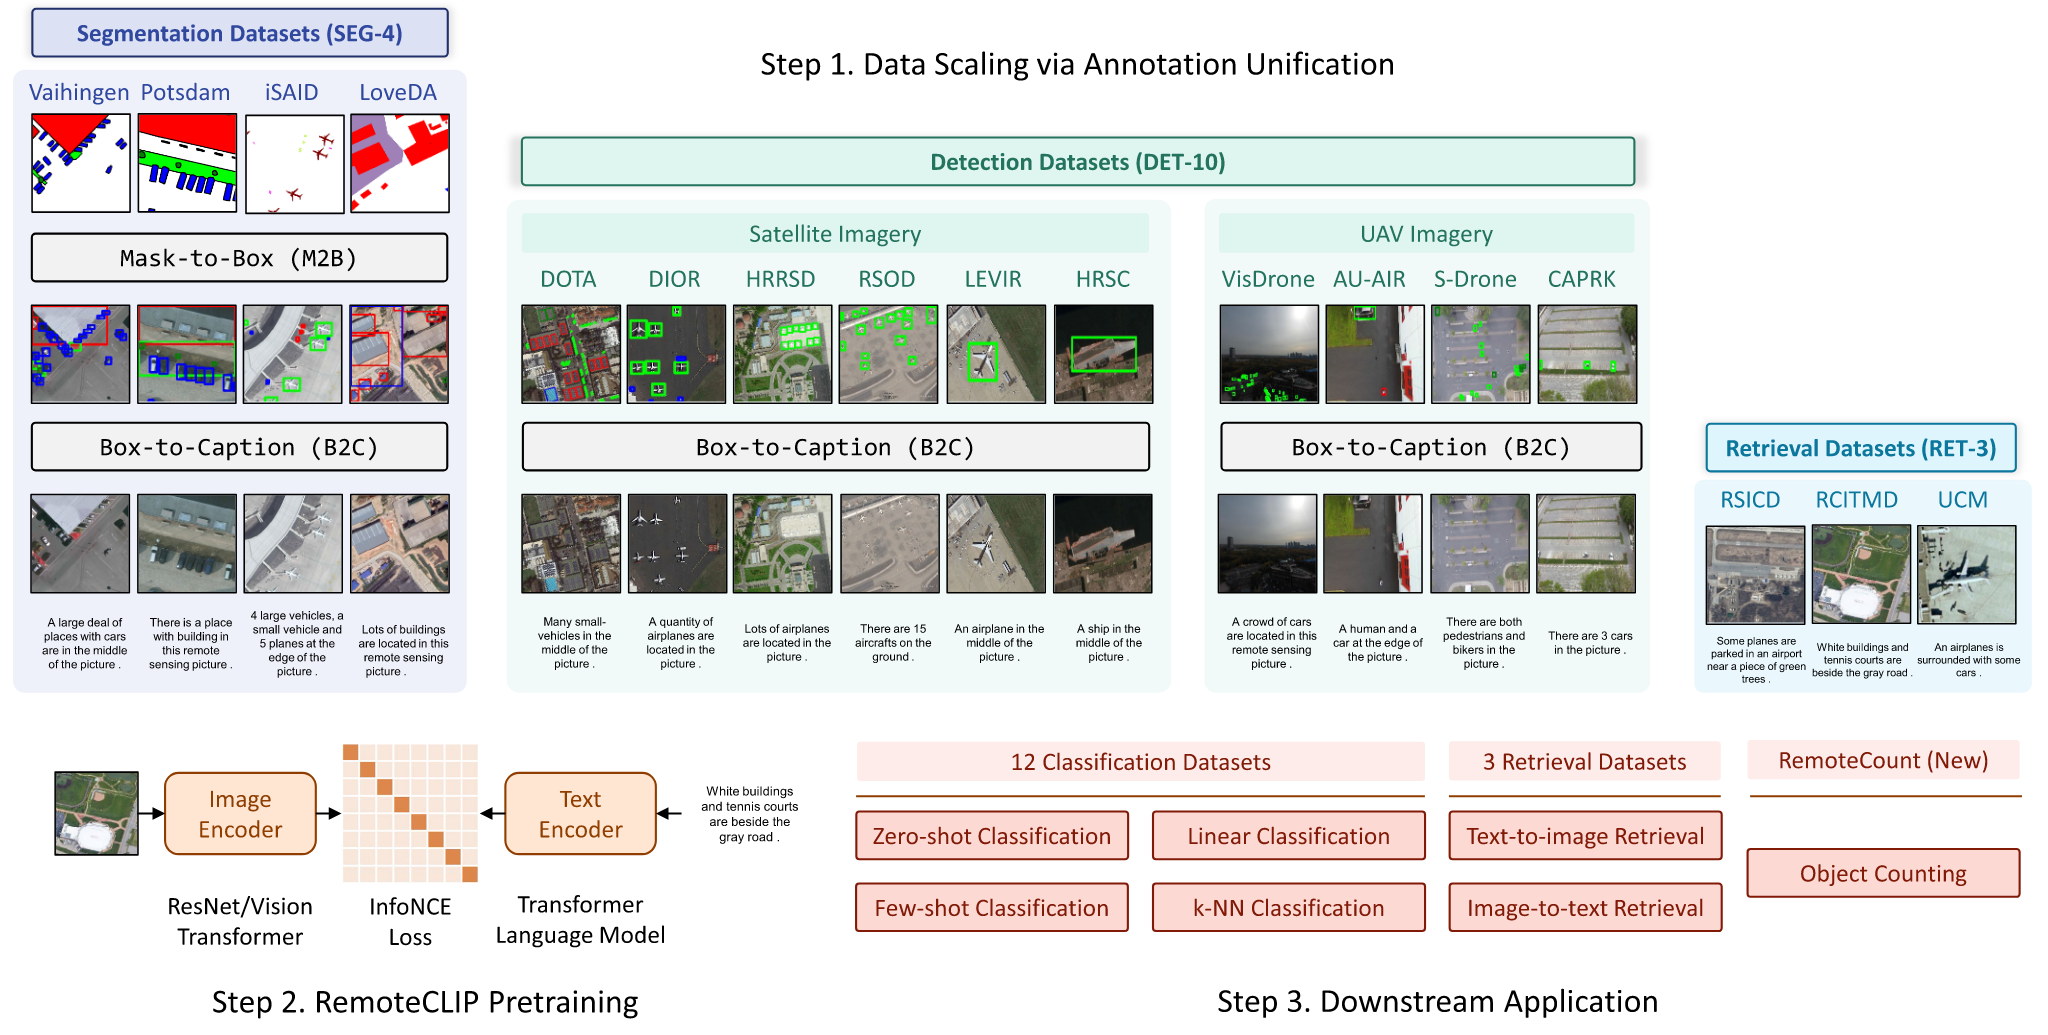
\includegraphics[width=0.8\linewidth]{remoteclip.png}
      \caption{\scriptsize RemoteCLIP~\parencite{liuRemoteCLIPVisionLanguage2024}:面向遥感的视觉-语言基础模型。}
    \end{figure}
    \bottomleftrefs
  \end{frame}
\end{refsection}

\begin{refsection}
  \begin{frame}{传统数据增强方法}
    \begin{itemize}
      \item \textbf{几何变换:} \textbf{旋转}、\textbf{翻转}(水平/垂直)、\textbf{缩放}、\textbf{平移}、\textbf{裁剪}
      \item \textbf{颜色扰动:} 调整亮度、对比度、饱和度和色调
      \item \textbf{噪声注入:} 向图像中添加随机噪声
      \item \textbf{Cutout}~\parencite{devriesImprovedRegularizationConvolutional2017}
      \item \textbf{CutMix}~\parencite{yunCutMixRegularizationStrategy2019}
      \item \textbf{Copy-Paste}~\parencite{ghiasiSimpleCopyPasteStrong2021}
    \end{itemize}
    还有一项系统性研究《How to train your ViT? Data, Augmentation,  and Regularization in Vision Transformers》~\parencite{steinerHowTrainYour2022}。
    \bottomleftrefs
  \end{frame}
\end{refsection}

\begin{refsection}
  \begin{frame}{用于数据增强的生成模型}
    \begin{figure}
      \centering
      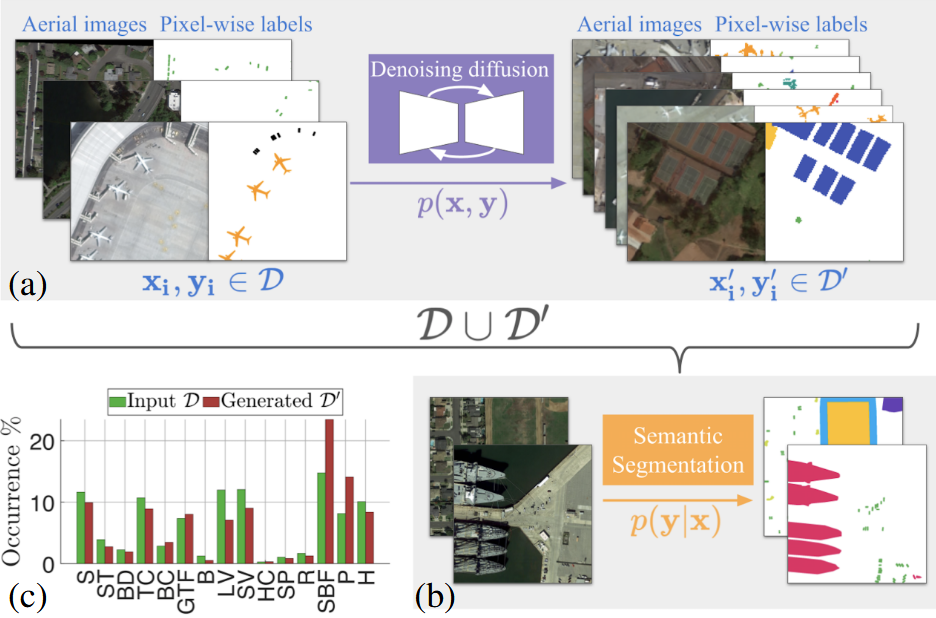
\includegraphics[height=0.6\textheight]{satsyn.png}
      
      \vspace{0.5em}
      \caption{\scriptsize SatSyn~\parencite{tokerSatSynthAugmentingImageMask2024} 提出了一种生成模型(扩散模型),可同时生成卫星分割的图像和对应掩码。该合成数据集用于数据增强,在卫星语义分割任务中相比其他增强方法带来了显著的定量提升。}
    \end{figure}

    \bottomleftrefs
  \end{frame}
\end{refsection}

\begin{refsection}
  \begin{frame}{生成的文本-图像数据集提升图像分类}
    \centering
    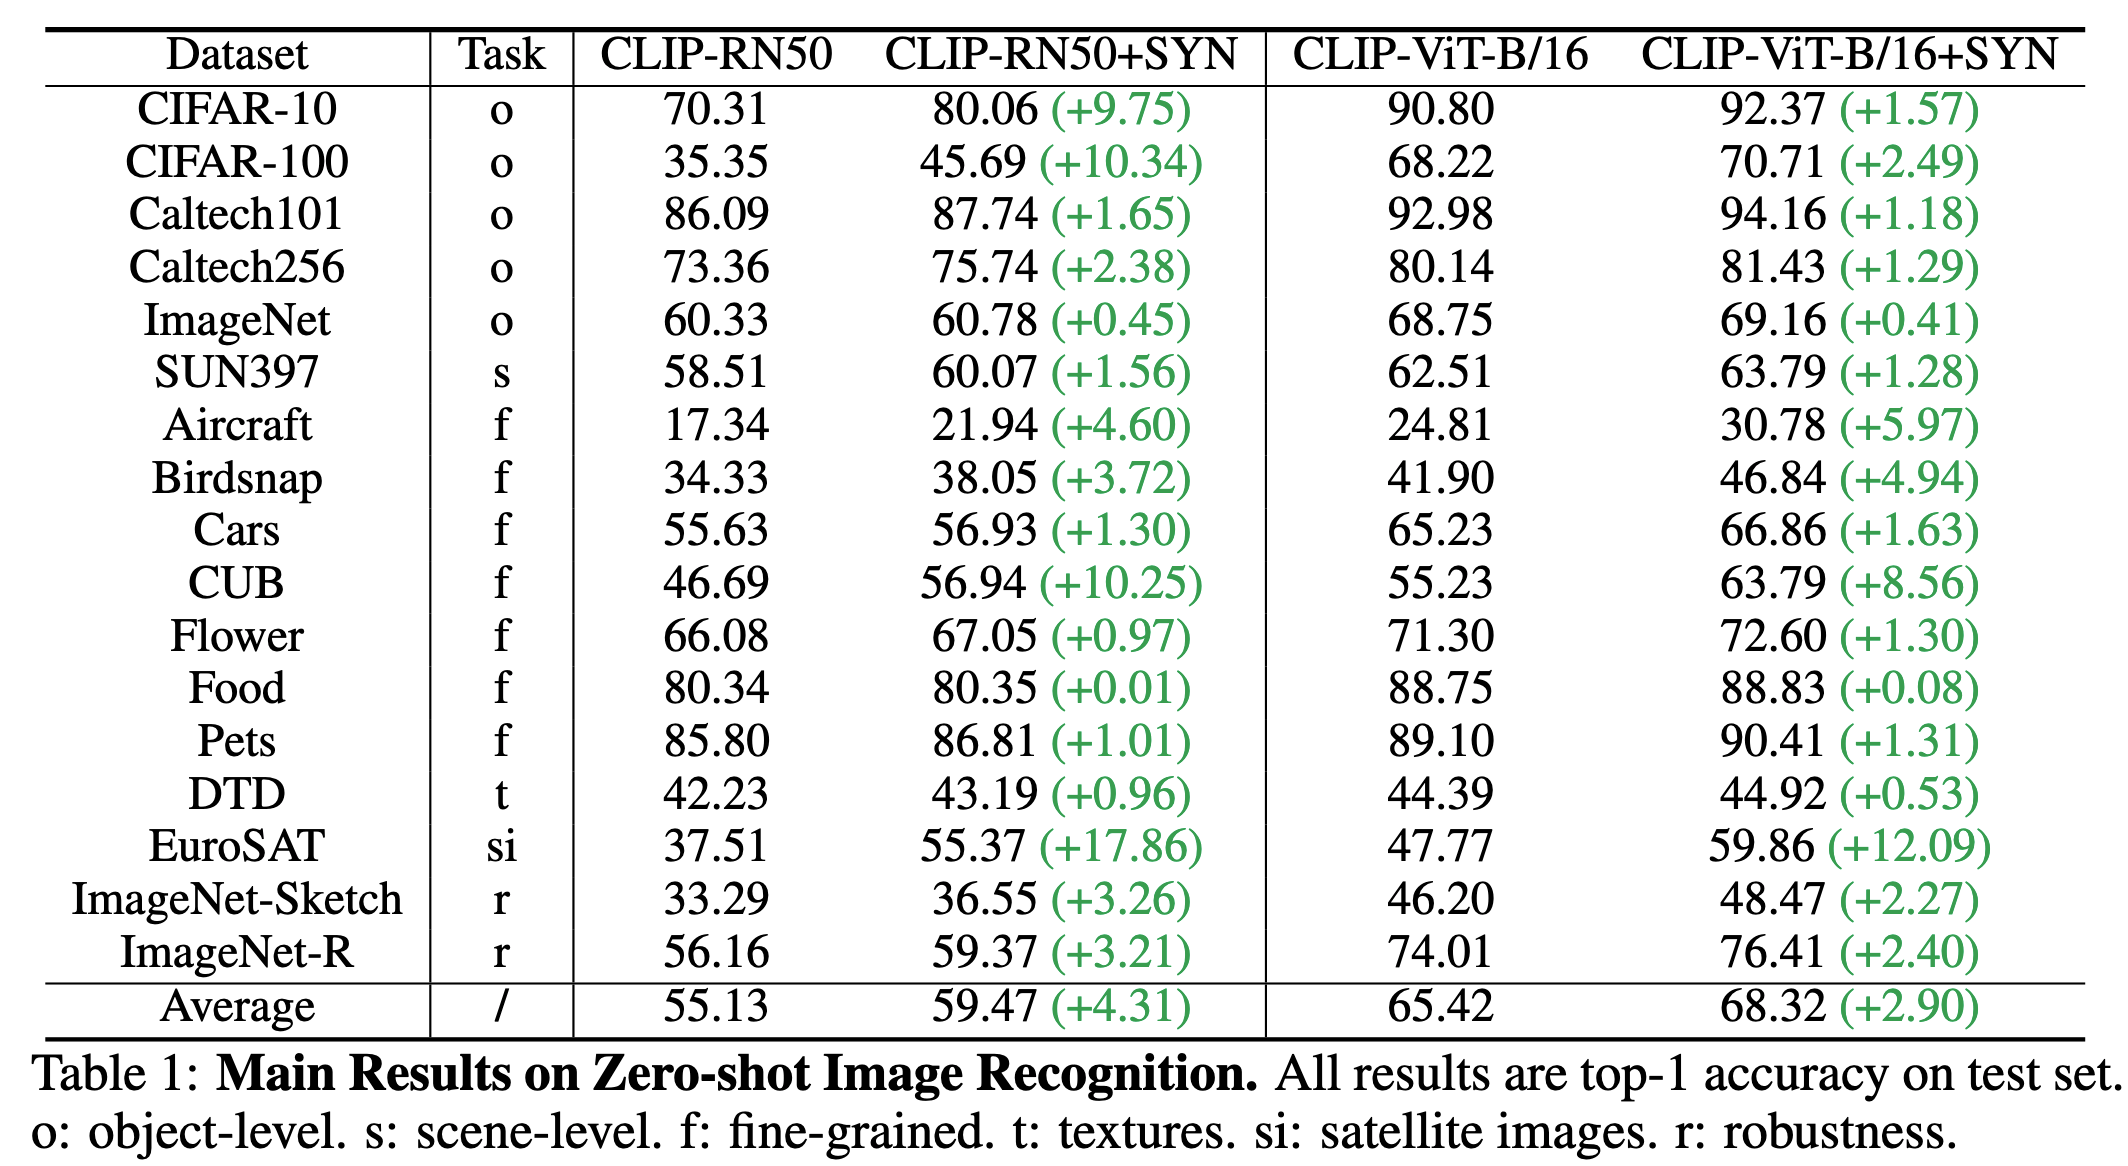
\includegraphics[width=0.8\linewidth]{syn_aug_results.png}
    
    % \vspace{0.5em}
    
    \scriptsize
    由生成模型合成的文本-图像数据集可显著提升图像分类性能,见~\parencite{heSYNTHETICDATAGENERATIVE2022}。
    \bottomleftrefs
  \end{frame}
\end{refsection}

\begin{refsection}
  \begin{frame}{xBD:大规模灾害损失数据集}
    \centering
    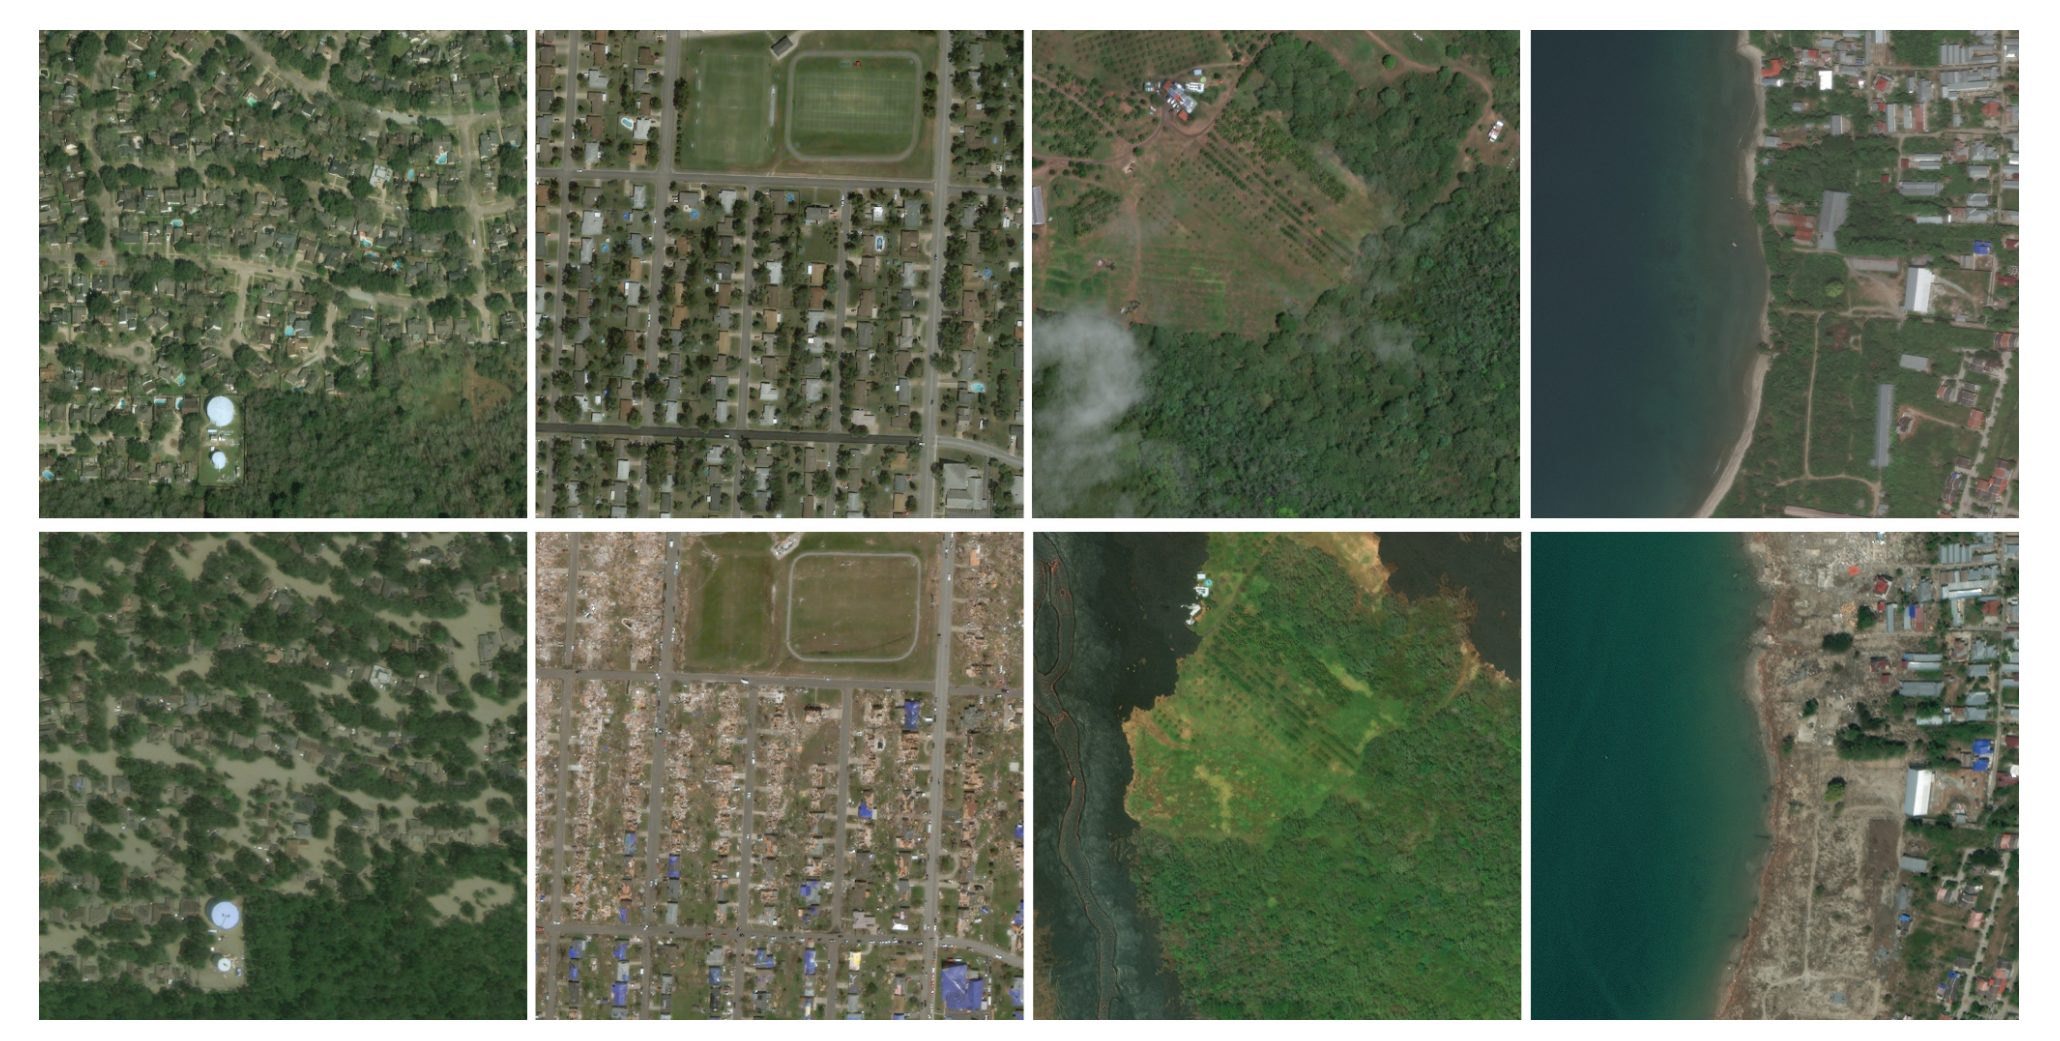
\includegraphics[width=0.85\linewidth]{xbd_samples.png}
    
    \vspace{0.5em}
    \scriptsize
    灾前影像(上)与灾后影像(下)。从左到右依次为:哈维飓风、乔普林龙卷风、下普纳火山喷发、巽他海峡海啸。影像来源:DigitalGlobe。\\
    \textbf{xBD}~\parencite{guptaCreatingXBDDataset2019}
    \bottomleftrefs
  \end{frame}
\end{refsection}

\begin{refsection}
  \begin{frame}{xBD:全球灾害类型覆盖}
    \centering
    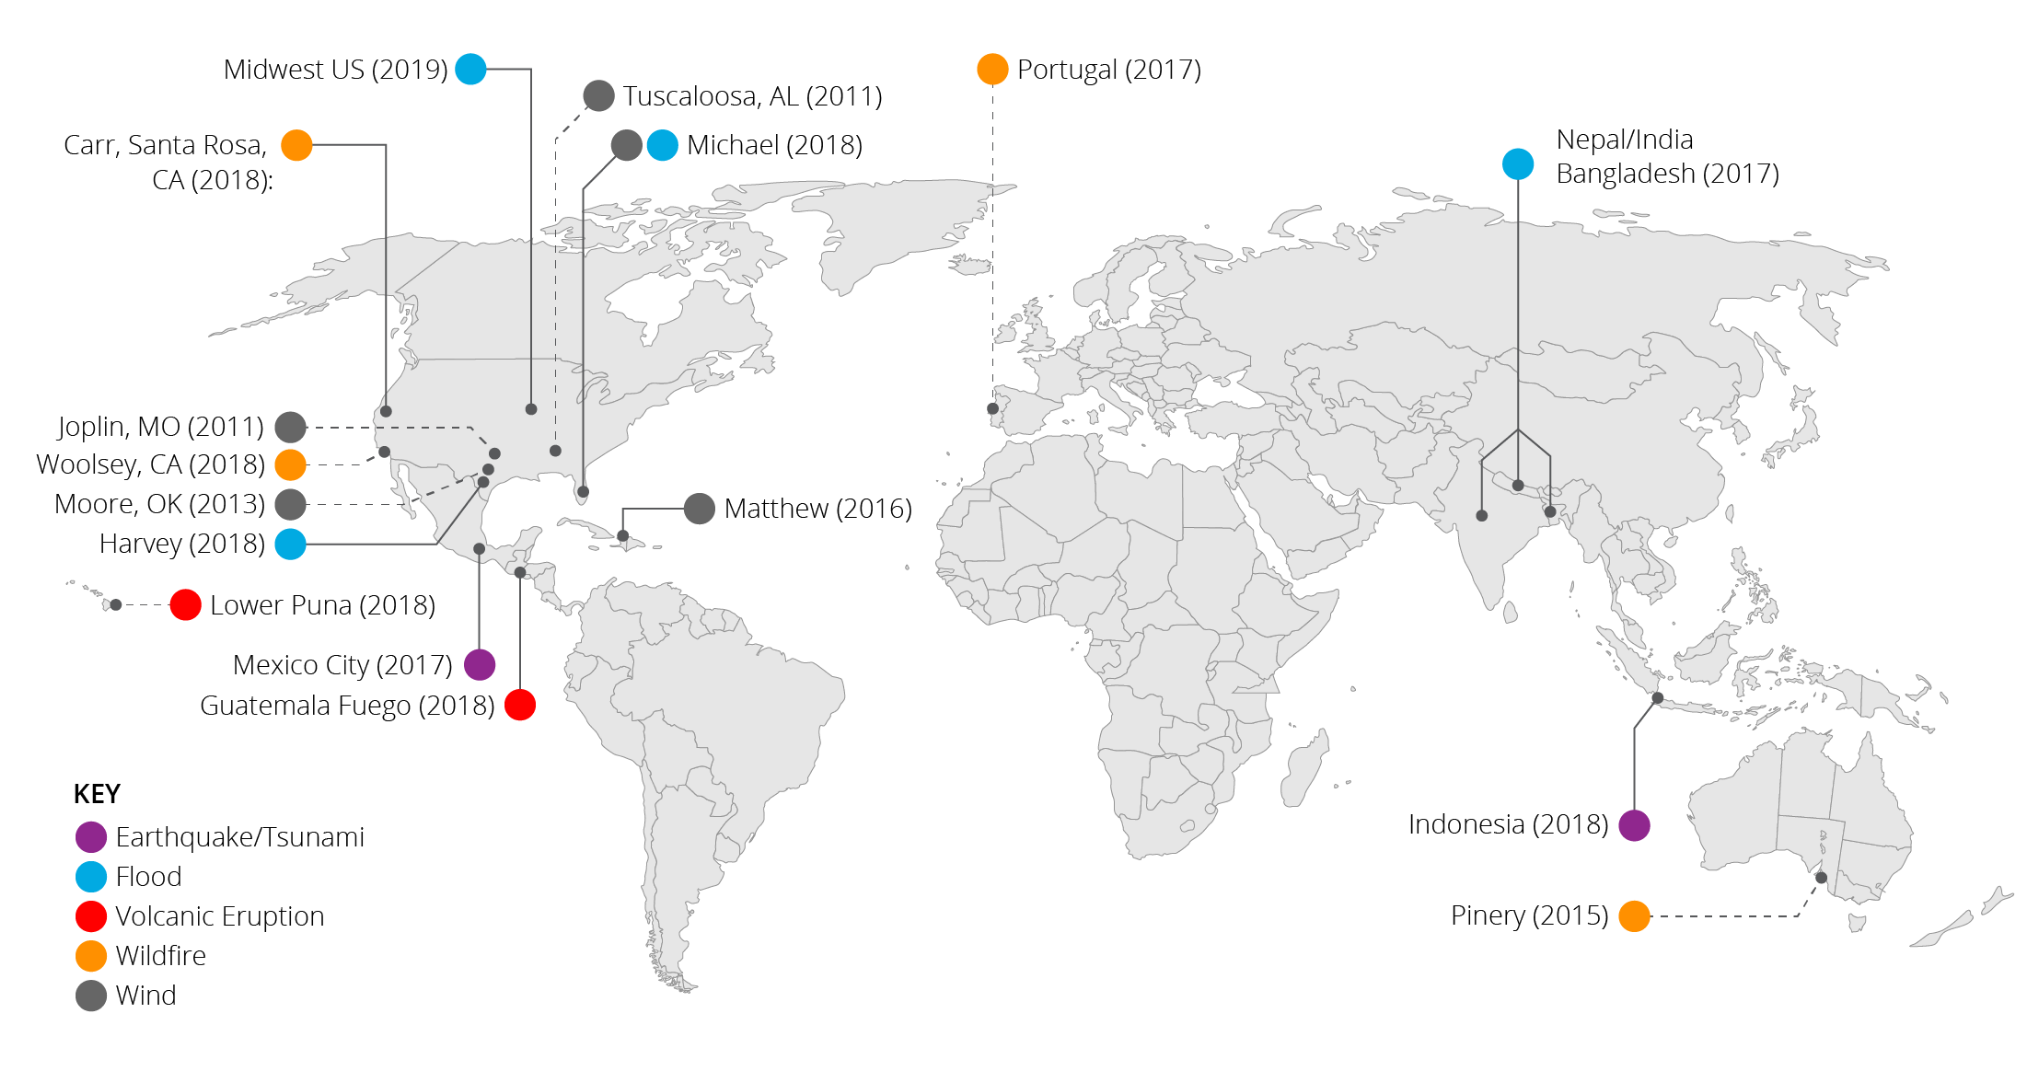
\includegraphics[width=0.85\linewidth]{xbd_global.png}
    
    \vspace{0.5em}
    \scriptsize
    xBD 数据集在全球范围内涵盖的灾害类型及事件。\\
    \textbf{xBD}~\parencite{guptaCreatingXBDDataset2019}
    \bottomleftrefs
  \end{frame}
\end{refsection}

\begin{refsection}
  \begin{frame}{场景分类与超分辨率的基线模型}
    \textbf{场景图像分类:}
    \begin{itemize}
      \item \textbf{CLIP}~\parencite{radfordLearningTransferableVisual2021}
      \item \textbf{RemoteCLIP}~\parencite{liuRemoteCLIPVisionLanguage2024}
      \item \textbf{Git-RSCLIP}~\parencite{text2earth2025}
    \end{itemize}
    \bottomleftrefs
  \end{frame}
\end{refsection}

%--- 幻灯片:文本到图像生成的数据集 ---
\begin{refsection}
  \begin{frame}{文本到图像生成的其他数据集}
    \textbf{文本到图像生成:}
    \begin{itemize}
      \item \textbf{RSICD}~\parencite{lu2017exploring}:遥感图像描述数据集,包含10,921张图像,每张图像有5条描述。
      \item \textbf{RSICap}~\parencite{hu2023rsgpt}:高质量数据集,包含2,585个人工标注的图像-文本对。
      \item \textbf{UCM-Captions}~\parencite{qu2016deep}:基于UC Merced土地利用数据集,包含2,100张图像,每张配有5条描述。
    \end{itemize}
    \bottomleftrefs
  \end{frame}
\end{refsection}

\begin{refsection}
  \begin{frame}[plain]
    \vfill
    \centering
    {\Huge \textbf{附录}}
    \vfill
  \end{frame}
\end{refsection}

\begin{refsection}
  \begin{frame}{生成建模}
    \begin{figure}
      \centering
      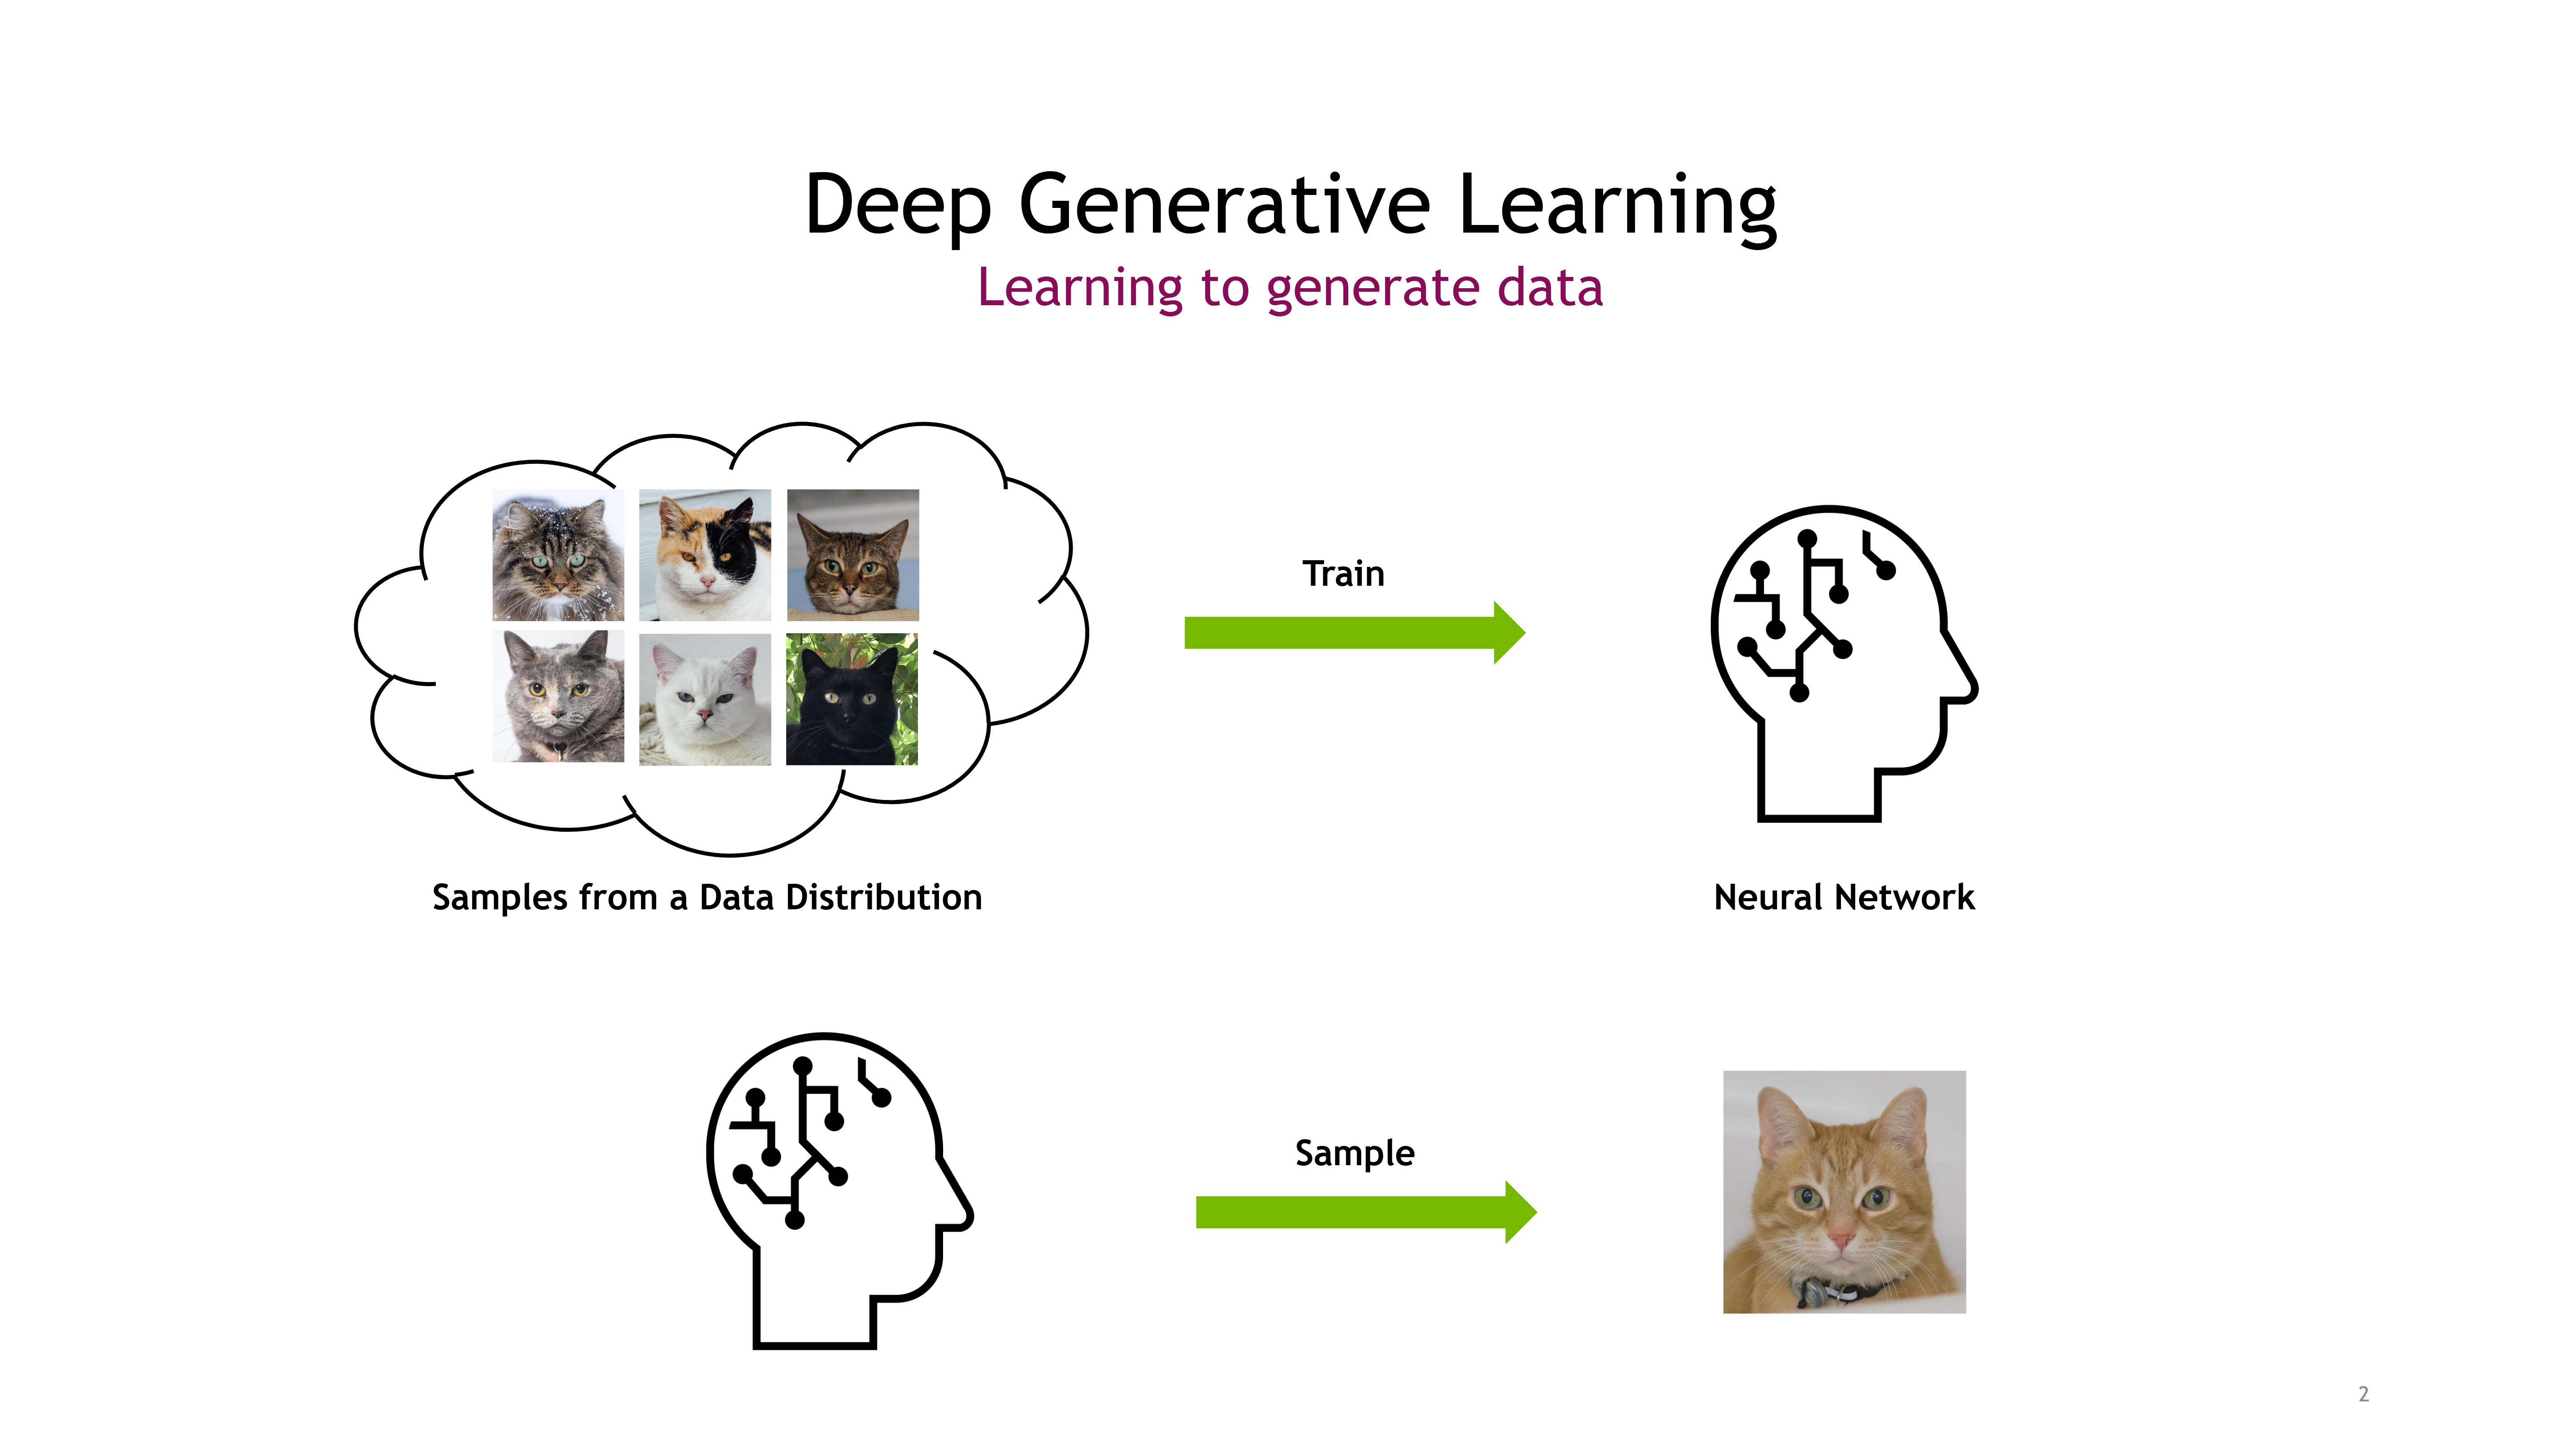
\includegraphics[width=0.8\linewidth]{learning_to_generate_data.png}
      \caption{\scriptsize 生成建模示意图~\parencite{CVPR2023Tutorial}。}
    \end{figure}
    \bottomleftrefs
  \end{frame}
\end{refsection}

% --- 幻灯片 2: 生成模型发展时间线 ---
\begin{refsection}
\begin{frame}{生成模型发展时间线}
  \begin{figure}
    \centering
    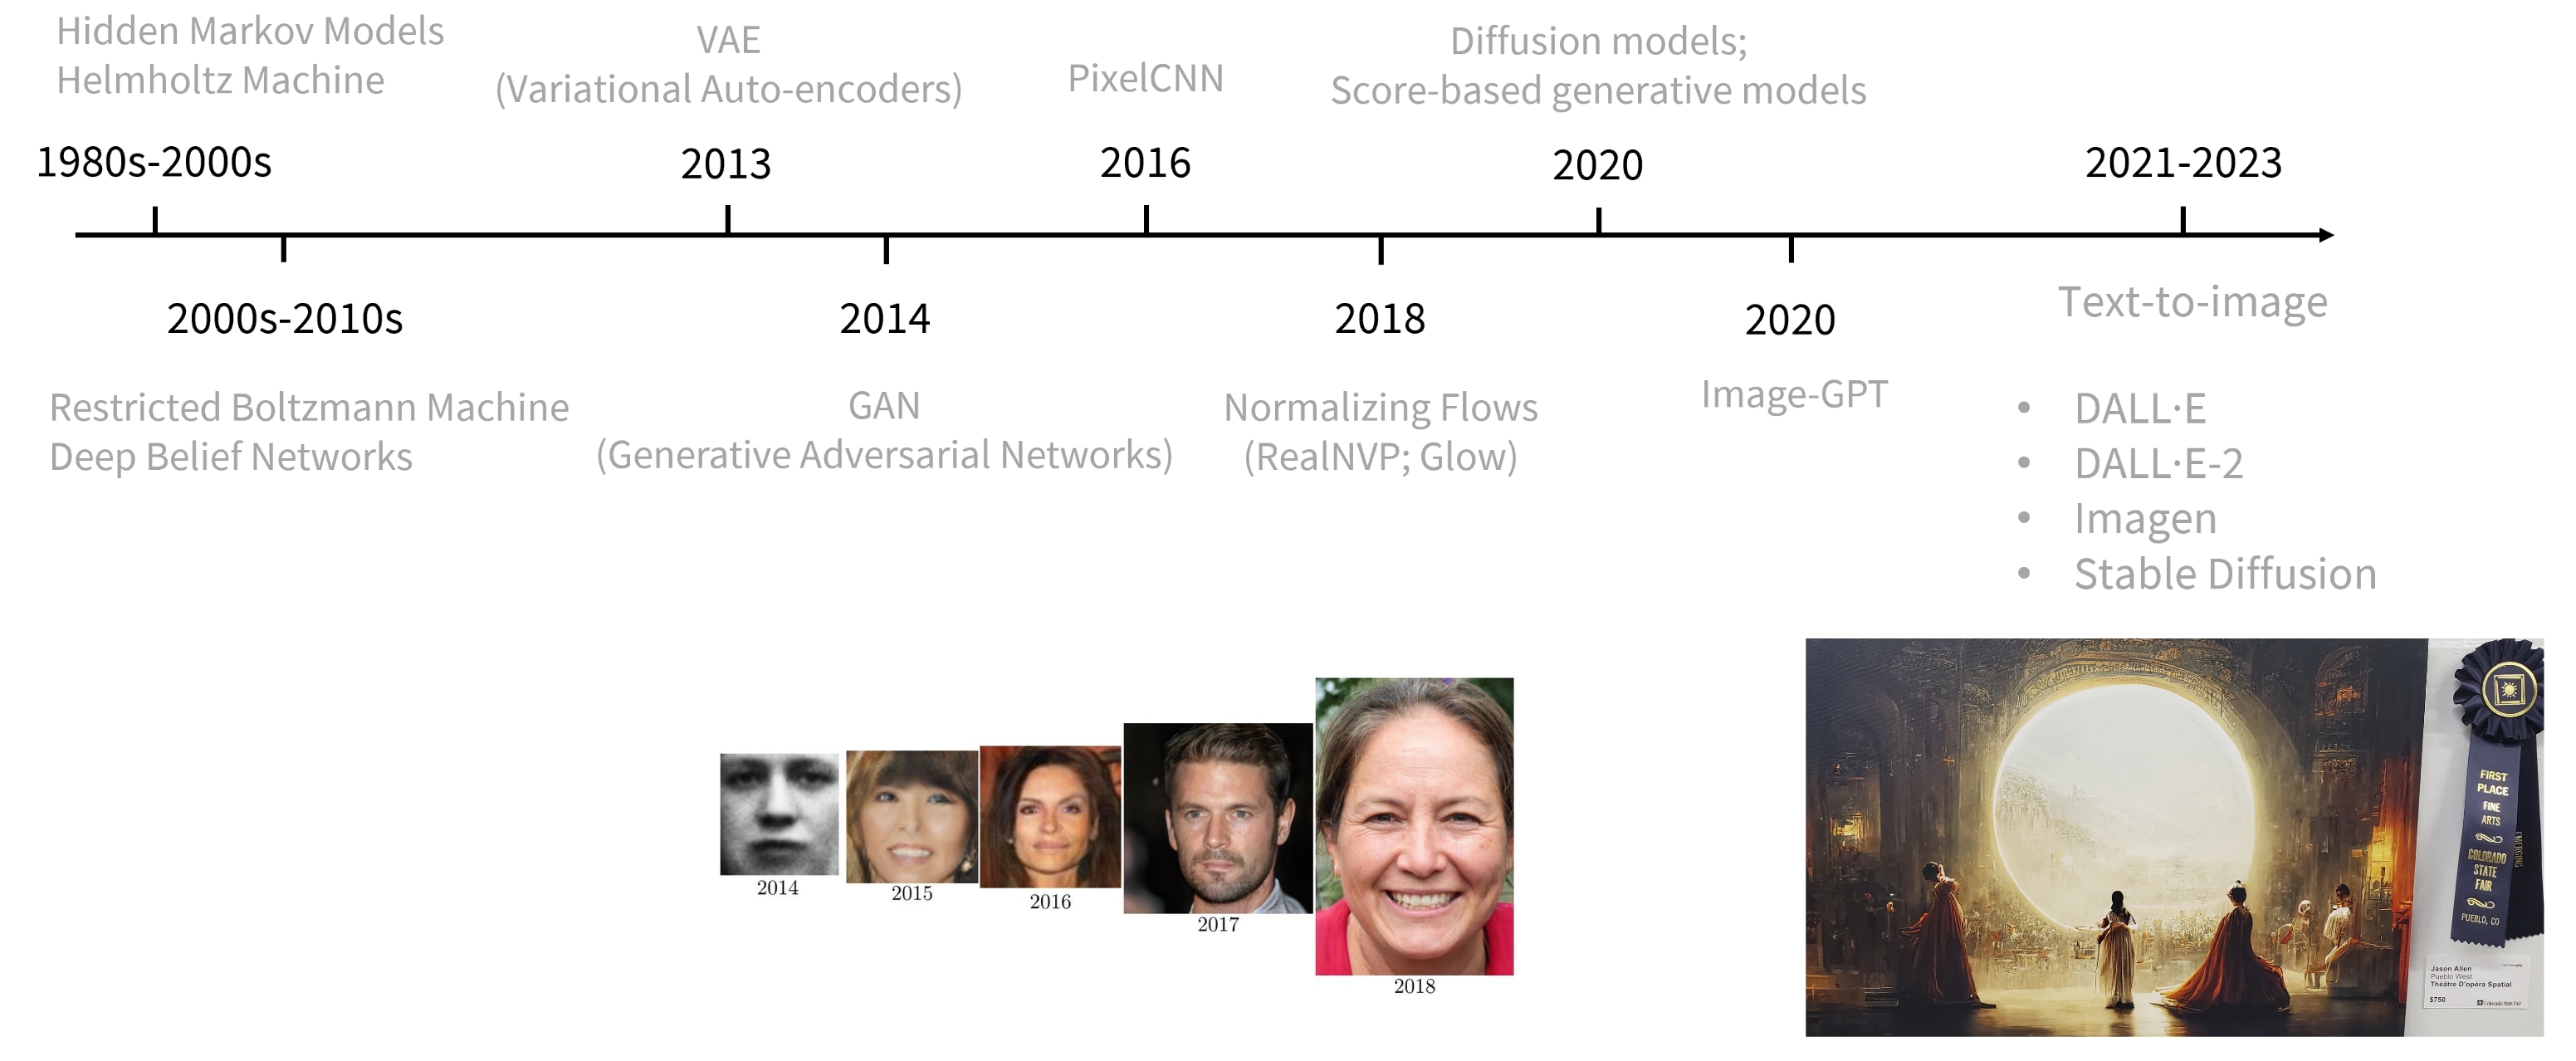
\includegraphics[width=0.95\linewidth]{genai_timeline.png}
    \caption{\scriptsize 生成模型关键发展历程时间线~\parencite{dengPPTAdvancedNueralNetwork2024}。}
  \end{figure}
  \bottomleftrefs
\end{frame}
\end{refsection}



\begin{refsection}
\begin{frame}{背景:扩散模型}

  \begin{figure}
    \begin{minipage}{0.95\linewidth}
      \footnotesize
      \textbf{去噪扩散模型包含两个过程:}
      \begin{itemize}
        \item 正向扩散过程:逐步向输入添加噪声
        \item 反向去噪过程:通过去噪学习生成数据
      \end{itemize}
    \end{minipage}
    \vspace{2em}

    \centering
    \includegraphics[width=1.0\linewidth]{diffusion_high_level.png}

    \caption[]{\scriptsize 扩散模型通过迭代去噪生成数据~\parencite{sohl2015deep,ho2020denoising}。}
  \end{figure}

  \bottomleftrefs
\end{frame}
\end{refsection}

% --- 幻灯片 4: 扩散模型原理 ---
\begin{refsection}
\begin{frame}{扩散模型:正向与反向过程}
  \footnotesize
  \textbf{正向(扩散)过程:}
  \begin{align*}
    q(\mathbf{x}_t \mid \mathbf{x}_{t-1}) &= \mathcal{N}(\mathbf{x}_t; \sqrt{1-\beta_t}\,\mathbf{x}_{t-1}, \beta_t \mathbf{I}) \\
    q(\mathbf{x}_{1:T} \mid \mathbf{x}_0) &= \prod_{t=1}^T q(\mathbf{x}_t \mid \mathbf{x}_{t-1}) \\
    &\text{等价于} 
    \mathbf{x}_t = \sqrt{\bar{\alpha}_t}\,\mathbf{x}_0 + \sqrt{1-\bar{\alpha}_t}\,\boldsymbol{\epsilon}, \quad \boldsymbol{\epsilon} \sim \mathcal{N}(\mathbf{0}, \mathbf{I})
  \end{align*}

  \footnotesize
  \textbf{反向(去噪)过程:}
  \begin{align*}
    p_\theta(\mathbf{x}_{t-1} \mid \mathbf{x}_t) &= \mathcal{N}(\mathbf{x}_{t-1}; \boldsymbol{\mu}_\theta(\mathbf{x}_t, t), \Sigma_\theta(\mathbf{x}_t, t)) \\
    p_\theta(\mathbf{x}_{0:T}) &= p(\mathbf{x}_T) \prod_{t=1}^T p_\theta(\mathbf{x}_{t-1} \mid \mathbf{x}_t)
  \end{align*}
  \scriptsize
  其中 $\mathbf{x}_0$ 为原始数据,$\beta_t$ 为噪声调度,$\bar{\alpha}_t = \prod_{s=1}^t (1-\beta_s)$。$p(\mathbf{x}_T) = \mathcal{N}(\mathbf{0}, \mathbf{I})$。

  \scriptsize
  \textbf{扩散模型通过学习逆转逐步加噪过程来生成数据。}~\parencite{sohl2015deep,ho2020denoising}
  \bottomleftrefs
\end{frame}
\end{refsection}

\begin{refsection}
\begin{frame}{扩散模型:训练与推理}
  \footnotesize
  \textbf{训练目标:}
  \begin{align*}
    \mathcal{L}_{\mathrm{simple}} = \mathbb{E}_{\mathbf{x}_0, \boldsymbol{\epsilon}, t} \left[ \left\| \boldsymbol{\epsilon} - \boldsymbol{\epsilon}_\theta(\sqrt{\bar{\alpha}_t}\mathbf{x}_0 + \sqrt{1-\bar{\alpha}_t}\boldsymbol{\epsilon}, t) \right\|^2 \right]
  \end{align*}
  其中 $\boldsymbol{\epsilon} \sim \mathcal{N}(\mathbf{0}, \mathbf{I})$,$\bar{\alpha}_t = \prod_{s=1}^t (1-\beta_s)$。

  \vspace{0.5em}
  \textbf{推理(采样):}
  \begin{itemize}
    \item 从纯噪声开始:$\mathbf{x}_T \sim \mathcal{N}(\mathbf{0}, \mathbf{I})$
    \item 对 $t = T, \ldots, 1$:
      \begin{itemize}
        \item 预测噪声:$\boldsymbol{\epsilon}_\theta(\mathbf{x}_t, t)$
        \item 计算均值:$\boldsymbol{\mu}_\theta(\mathbf{x}_t, t)$
        \item 采样:$\mathbf{x}_{t-1} \sim \mathcal{N}(\boldsymbol{\mu}_\theta(\mathbf{x}_t, t), \Sigma_\theta(\mathbf{x}_t, t))$
      \end{itemize}
    \item 重复直到得到 $\mathbf{x}_0$(生成样本)
  \end{itemize}

  \vspace{0.5em}
  \scriptsize
  \textbf{训练:} 最小化简化目标~\parencite{ho2020denoising}。\\
  \textbf{推理:} 通过迭代去噪从随机噪声生成数据。
  \bottomleftrefs
\end{frame}
\end{refsection}

%--- 幻灯片 5: 遥感图像生成应用:DiffusionSat, CRS-Diff, Text2Earth ---

\begin{refsection}
  \begin{frame}{遥感图像生成应用:Text2Earth}
    \begin{figure}
      \centering
      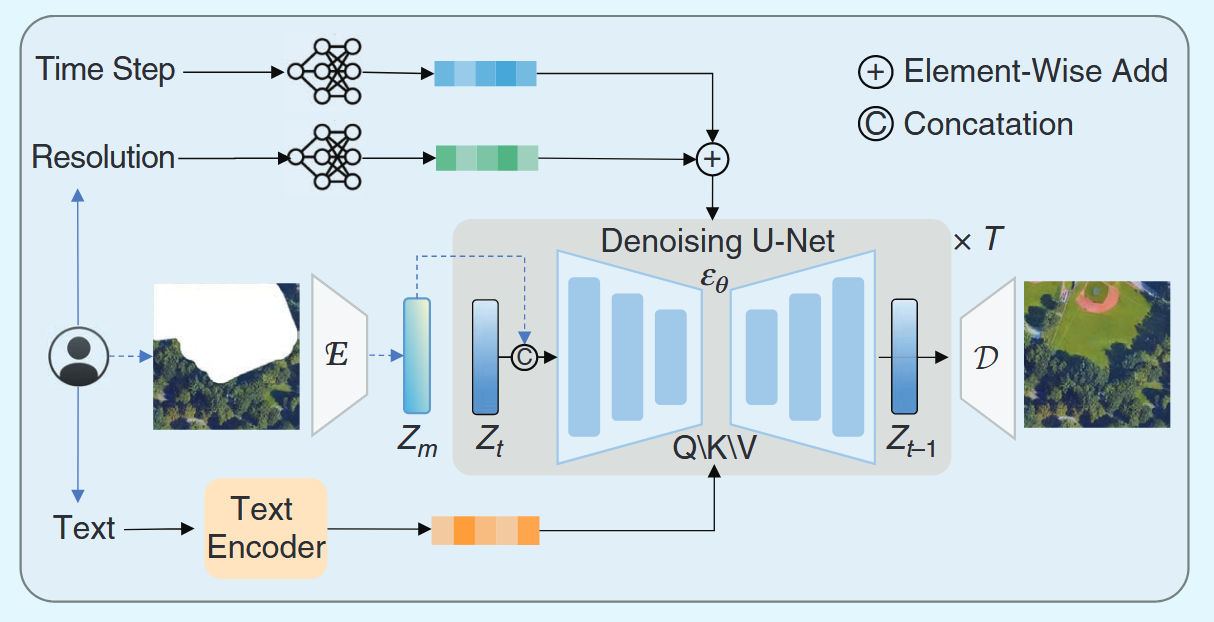
\includegraphics[width=0.9\linewidth]{text2earth.png}
      \caption[]{\scriptsize Text2Earth:面向文本驱动地球观测的基础模型~\parencite{text2earth2025}。}
    \end{figure}
    \bottomleftrefs
  \end{frame}
\end{refsection}

\begin{refsection}
  \begin{frame}{Text2Earth:生成结果示例}
    \begin{figure}
      \centering
      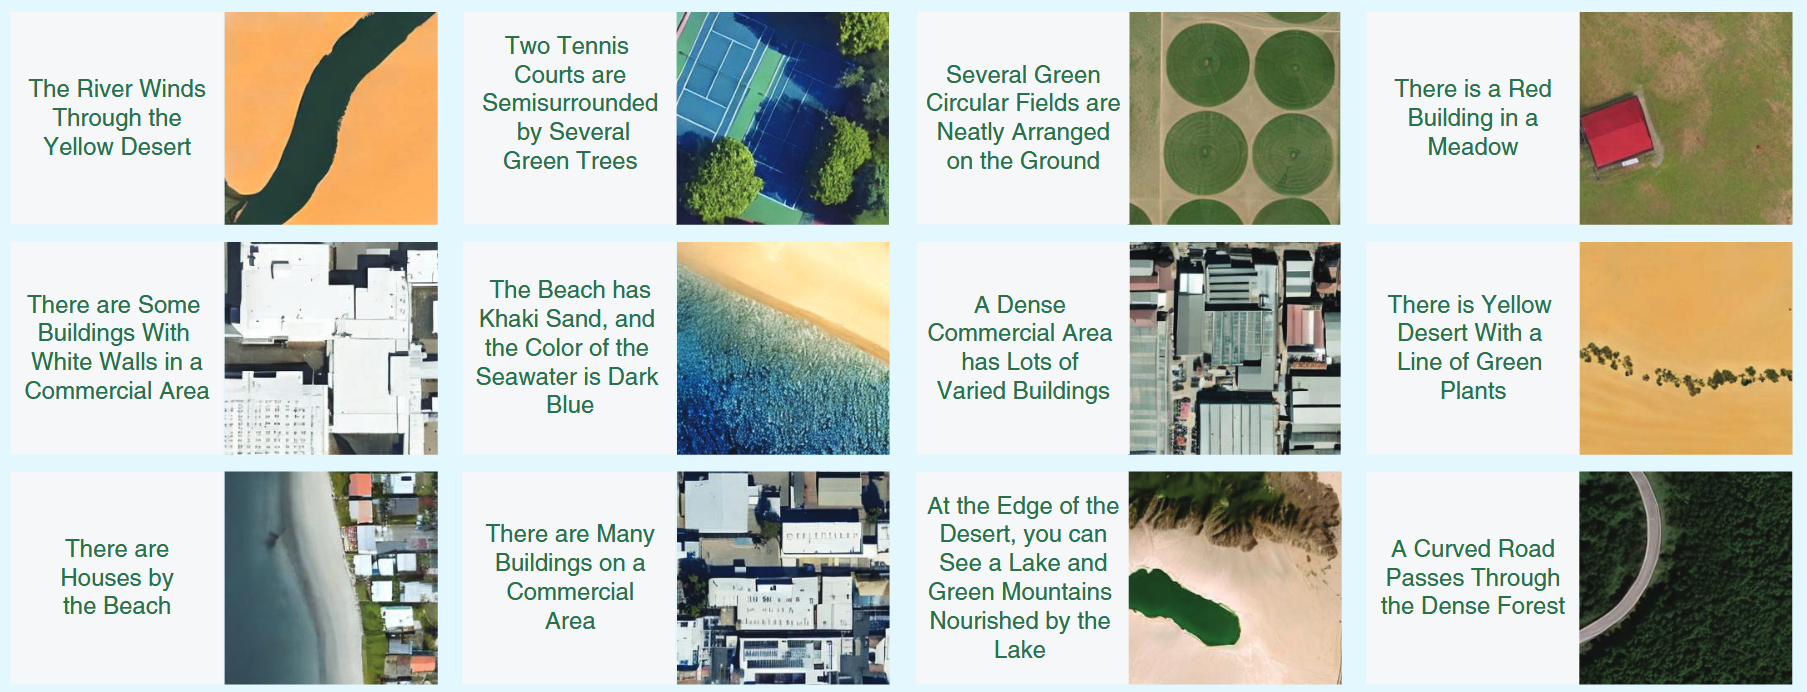
\includegraphics[width=0.9\linewidth]{text2earth_results.png}
      \caption[]{\scriptsize Text2Earth 生成的示例结果~\parencite{text2earth2025}。}
    \end{figure}
    \bottomleftrefs
  \end{frame}
\end{refsection}

\begin{refsection}
\begin{frame}{遥感图像生成应用:CRS-Diff}
  \begin{figure}
    \centering
    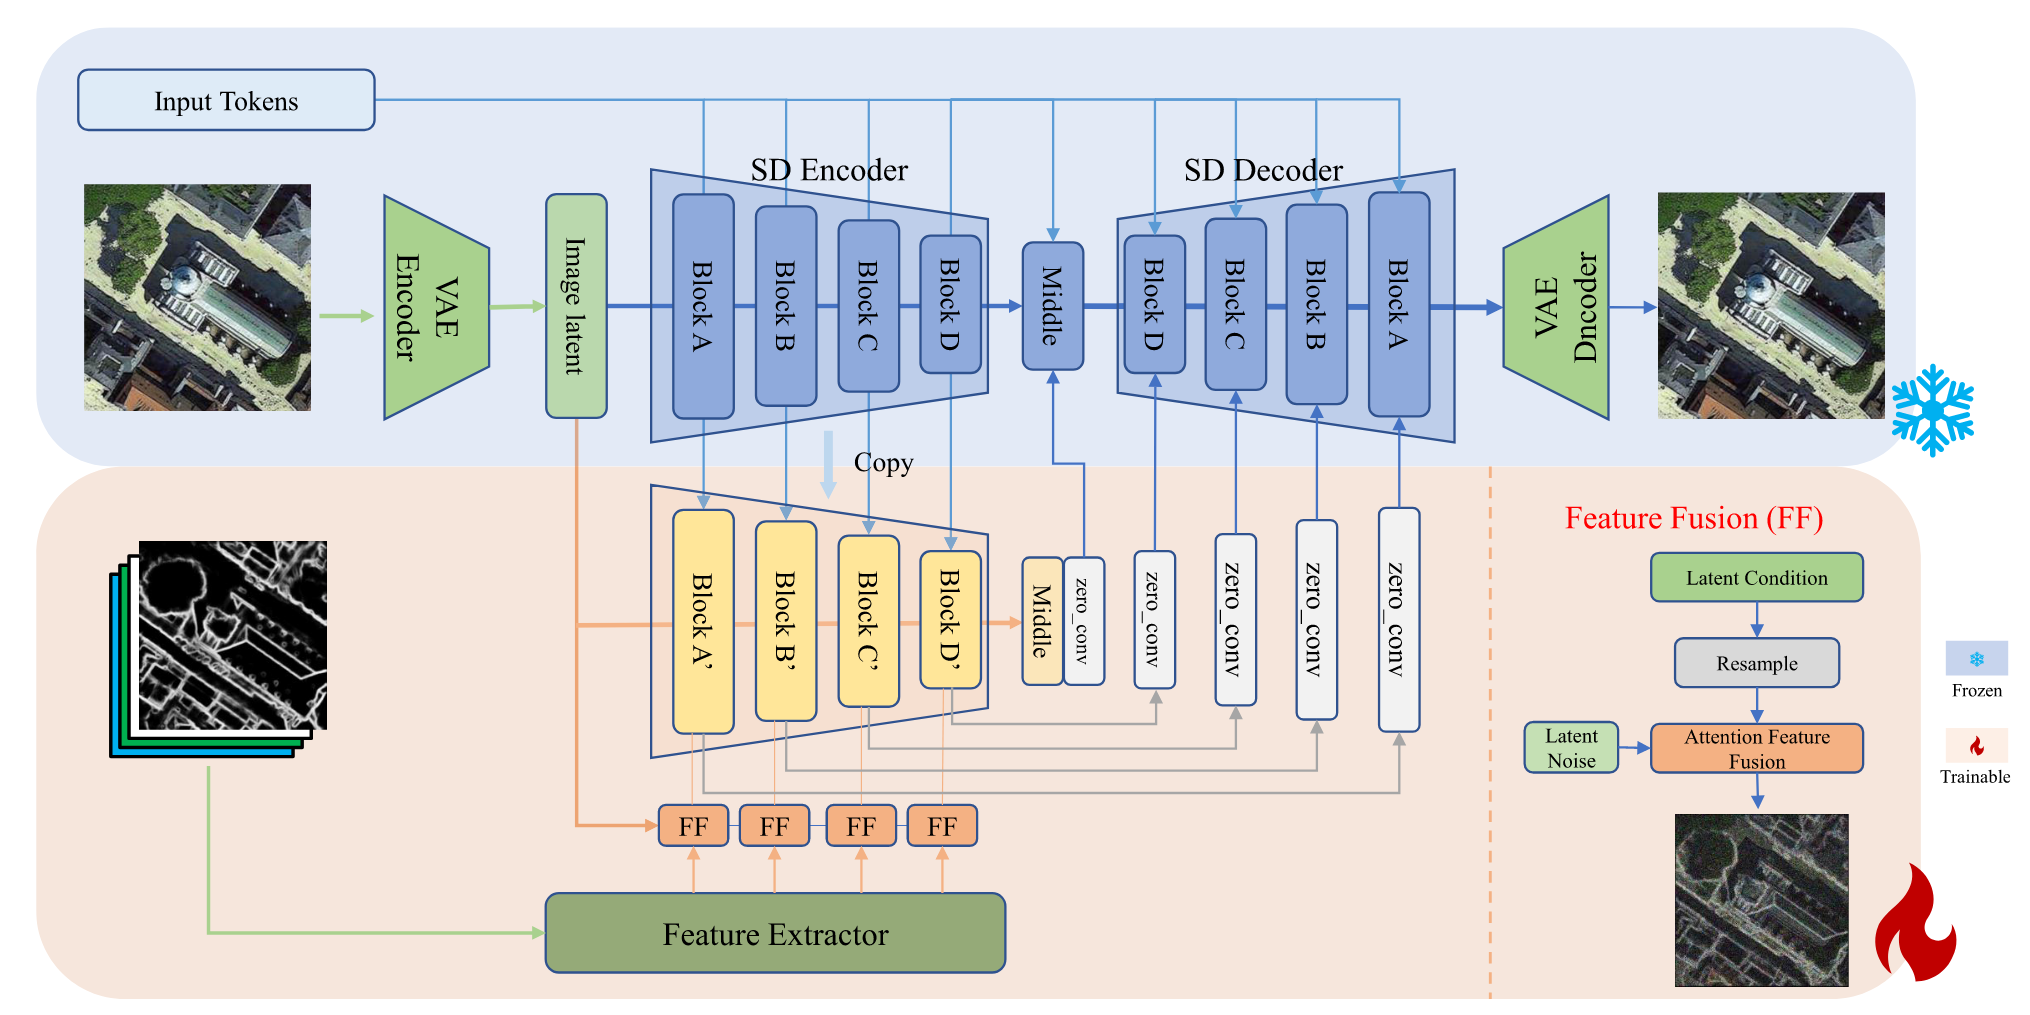
\includegraphics[width=0.9\linewidth]{crsdiff.png}
    \caption[]{\scriptsize CRS-Diff:可控遥感图像生成框架~\parencite{tang2024crsdiff}。}
  \end{figure}
  \bottomleftrefs
\end{frame}
\end{refsection}

\begin{refsection}
\begin{frame}{CRS-Diff:生成结果示例}
  \begin{figure}
    \centering
    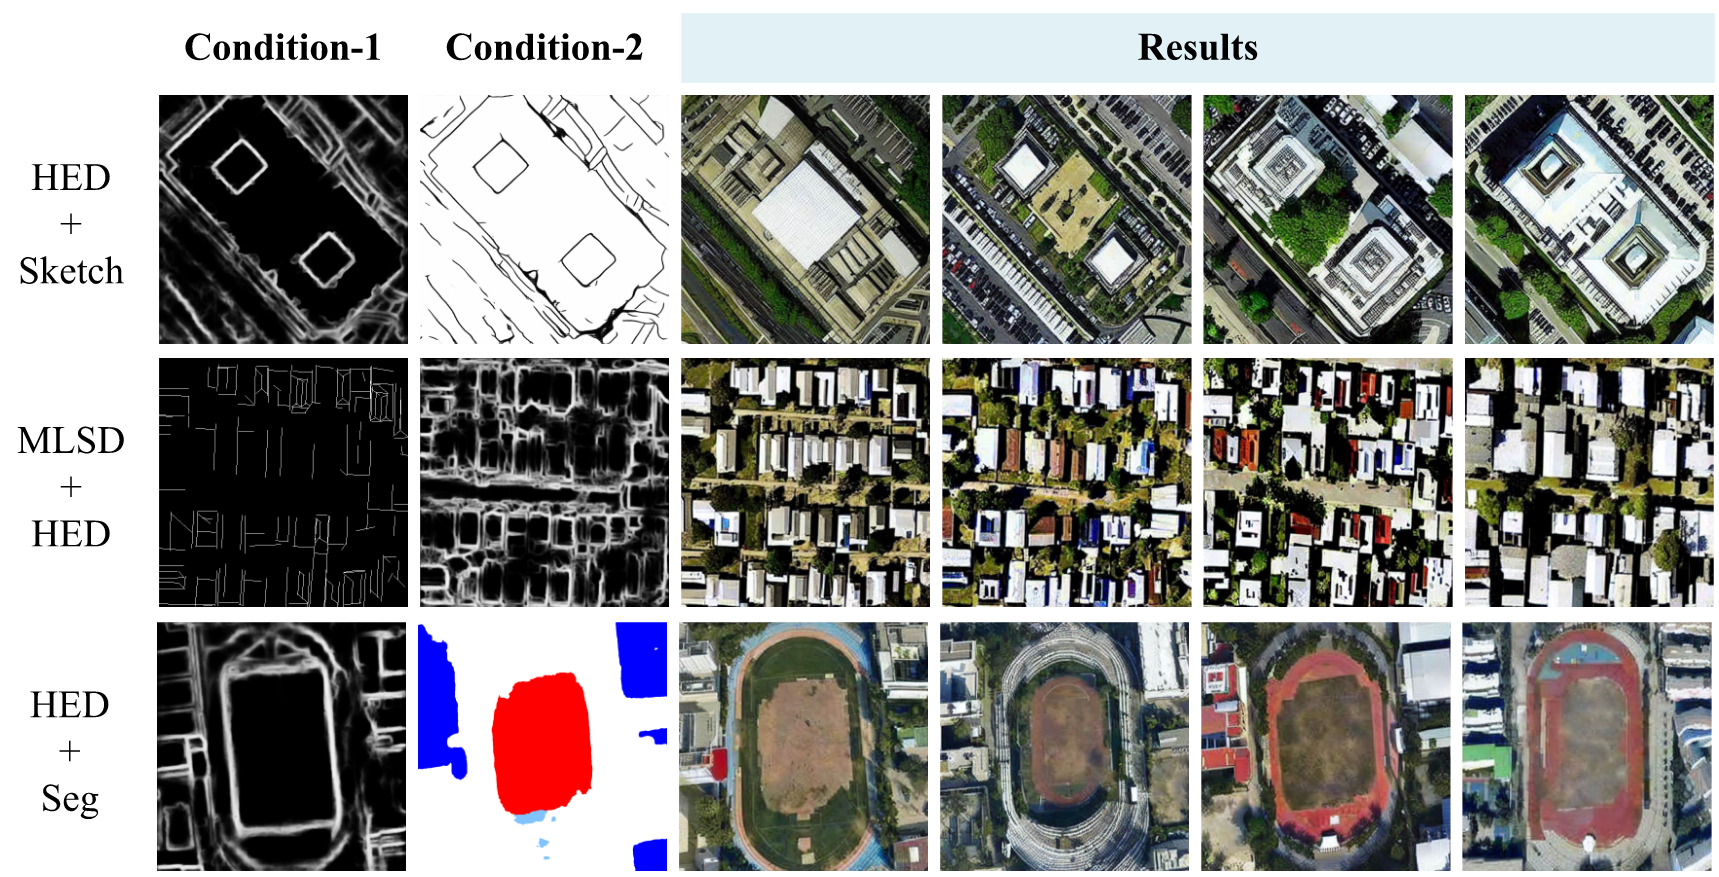
\includegraphics[width=0.9\linewidth]{crsdiff_results.png}
    \caption[]{\scriptsize CRS-Diff 生成的示例结果~\parencite{tang2024crsdiff}。}
  \end{figure}
  \bottomleftrefs
\end{frame}
\end{refsection}


%--- 幻灯片 6a: DiffusionSat 框架 ---
\begin{refsection}
\begin{frame}{DiffusionSat:框架概览}
  \begin{figure}
    \centering
    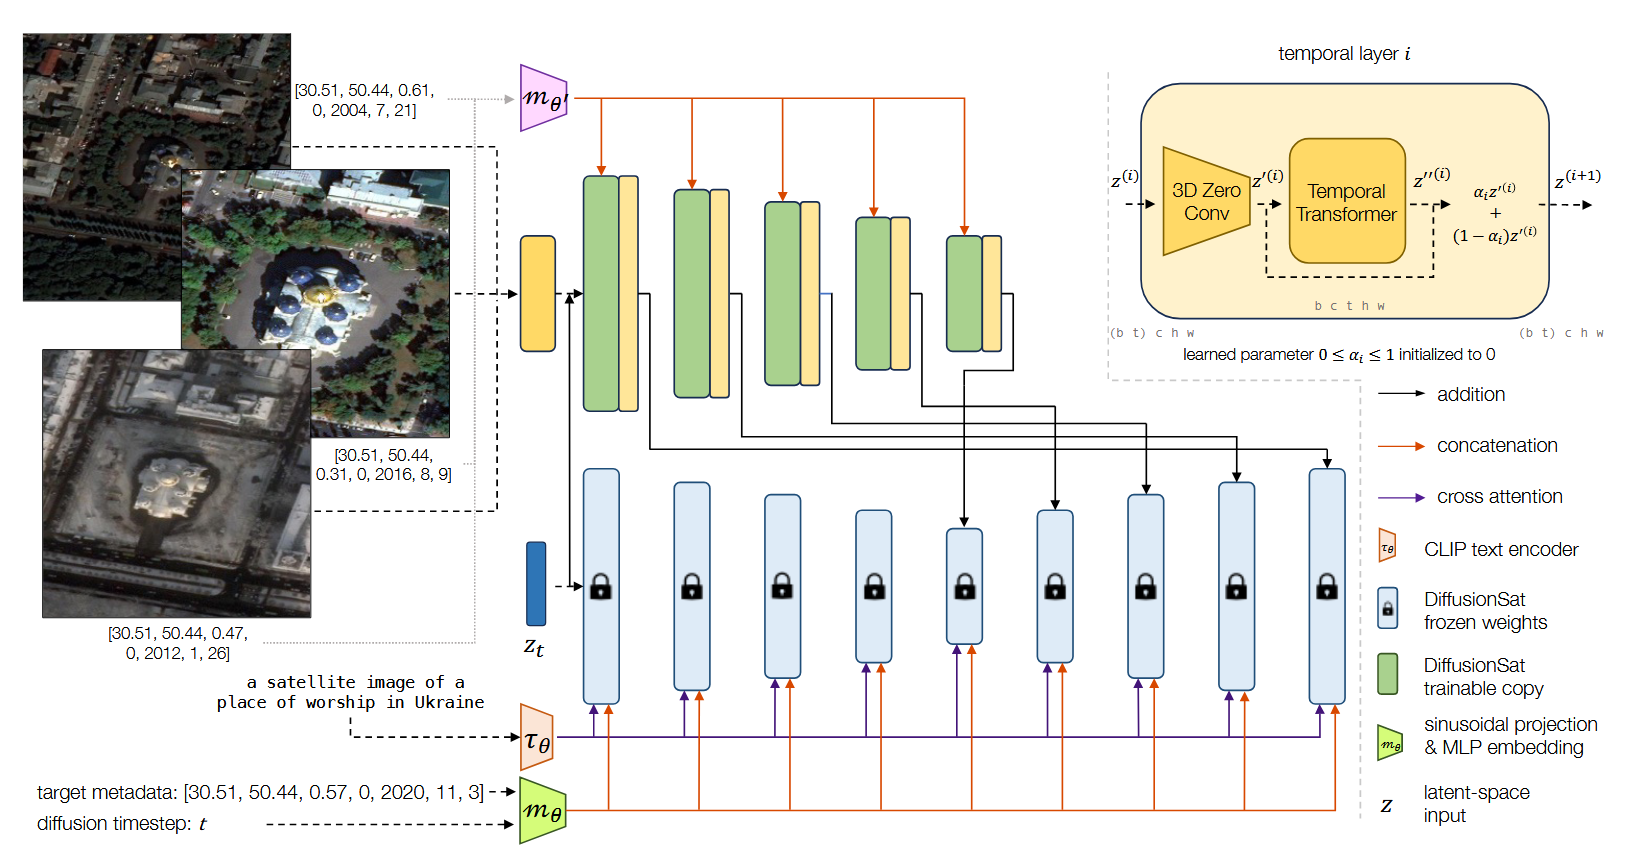
\includegraphics[width=0.9\linewidth]{diffusionsat.png}
    \caption[]{\scriptsize DiffusionSat:卫星影像生成基础模型~\parencite{diffusionset2024}。}
  \end{figure}
  \bottomleftrefs
\end{frame}
\end{refsection}

%--- 幻灯片 6b: DiffusionSat 超分辨率 ---
\begin{refsection}
\begin{frame}{DiffusionSat:多光谱超分辨率结果}
  \begin{figure}
    \centering
    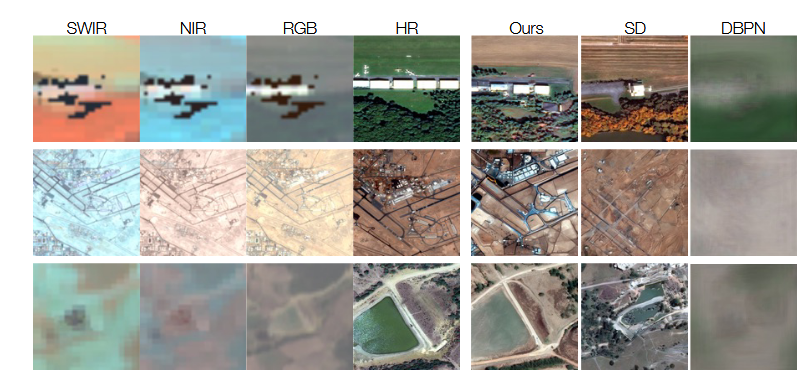
\includegraphics[width=0.9\linewidth]{diffusionsat_sr_results.png}
    \caption[]{\scriptsize DiffusionSat 多光谱超分辨率示例结果~\parencite{diffusionset2024}。}
  \end{figure}
  \bottomleftrefs
\end{frame}
\end{refsection}

%--- 幻灯片 6c: DiffusionSat 修复 ---
\begin{refsection}
\begin{frame}{DiffusionSat:遥感图像修复结果}
  \begin{figure}
    \centering
    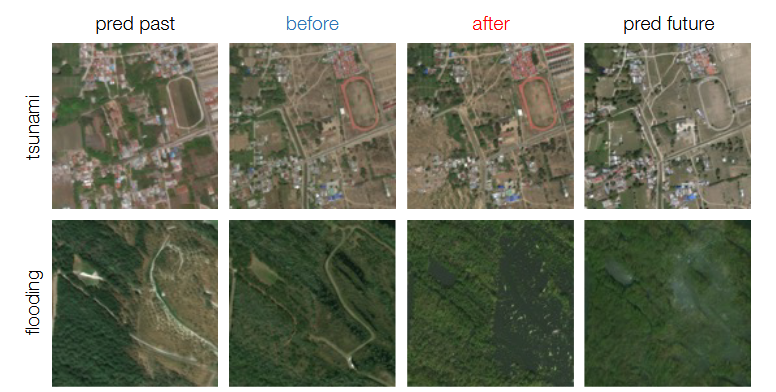
\includegraphics[width=0.9\linewidth]{diffusionsat_inpainting_results.png}
    \caption[]{\scriptsize DiffusionSat 遥感图像修复示例结果~\parencite{diffusionset2024}。}
  \end{figure}
  \bottomleftrefs
\end{frame}
\end{refsection}